% Controlled externalization protocol (replaces externalization_protocol.png).
%
% Usage in main.tex: requires the same preamble additions as
% pflc_formal_gap.tex (tikz + positioning, fit, backgrounds, arrows.meta, calc).
% Replace the existing 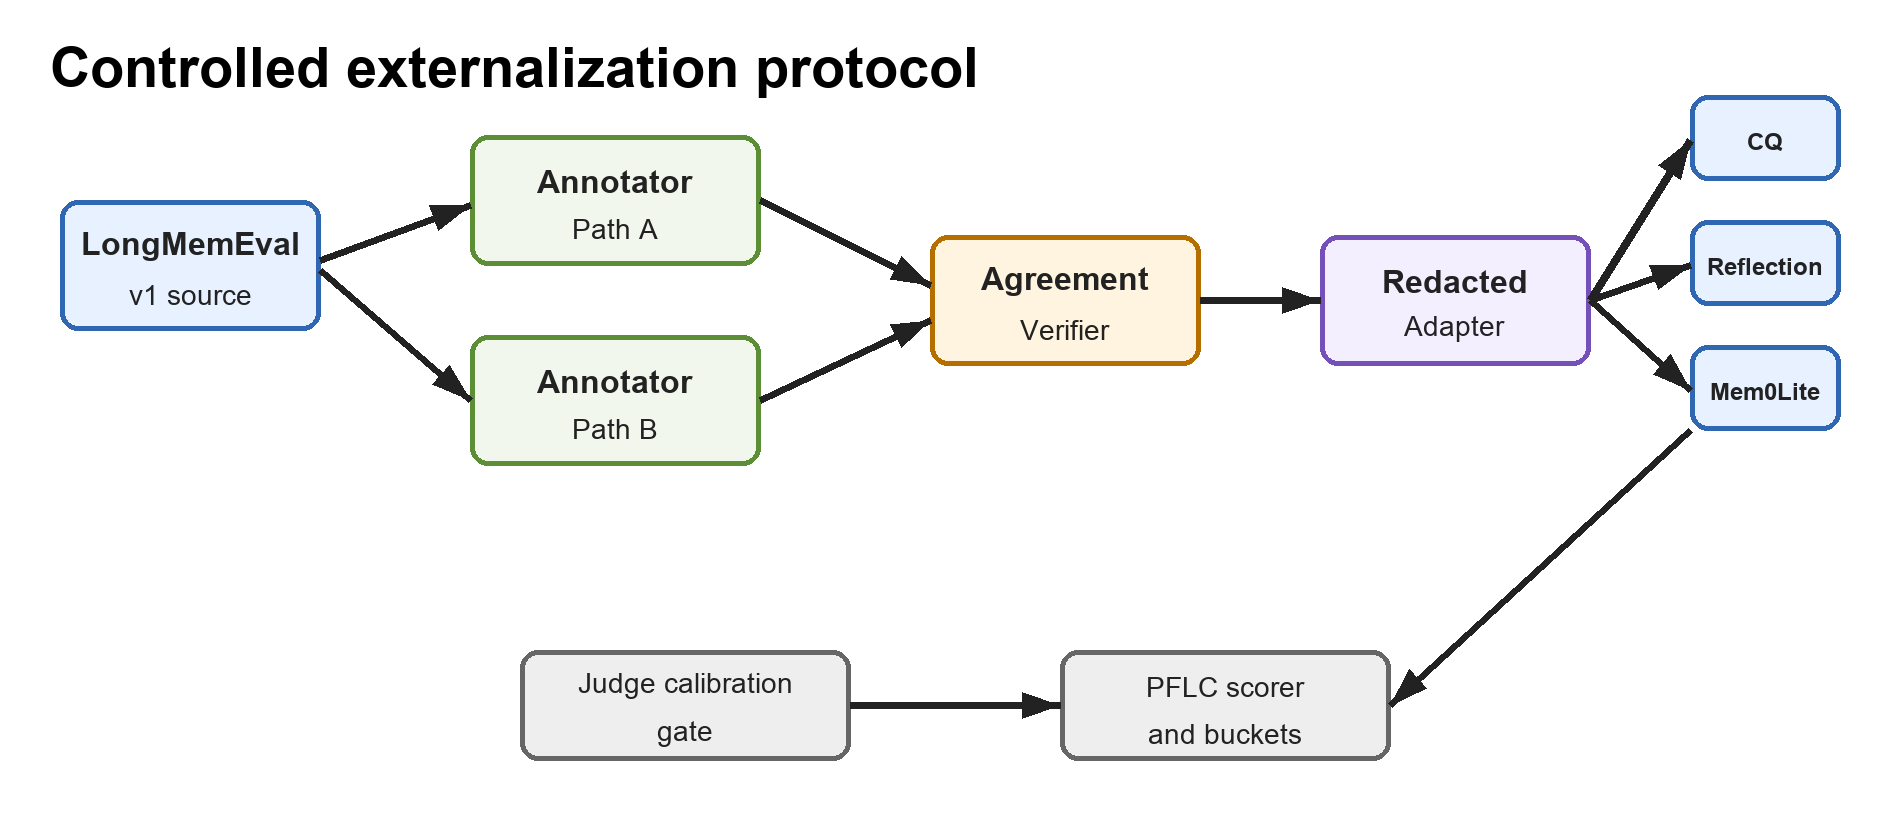
\includegraphics{figures/externalization_protocol.png}
% block in paper/sections/method.tex with
%   % Controlled externalization protocol (replaces externalization_protocol.png).
%
% Usage in main.tex: requires the same preamble additions as
% pflc_formal_gap.tex (tikz + positioning, fit, backgrounds, arrows.meta, calc).
% Replace the existing 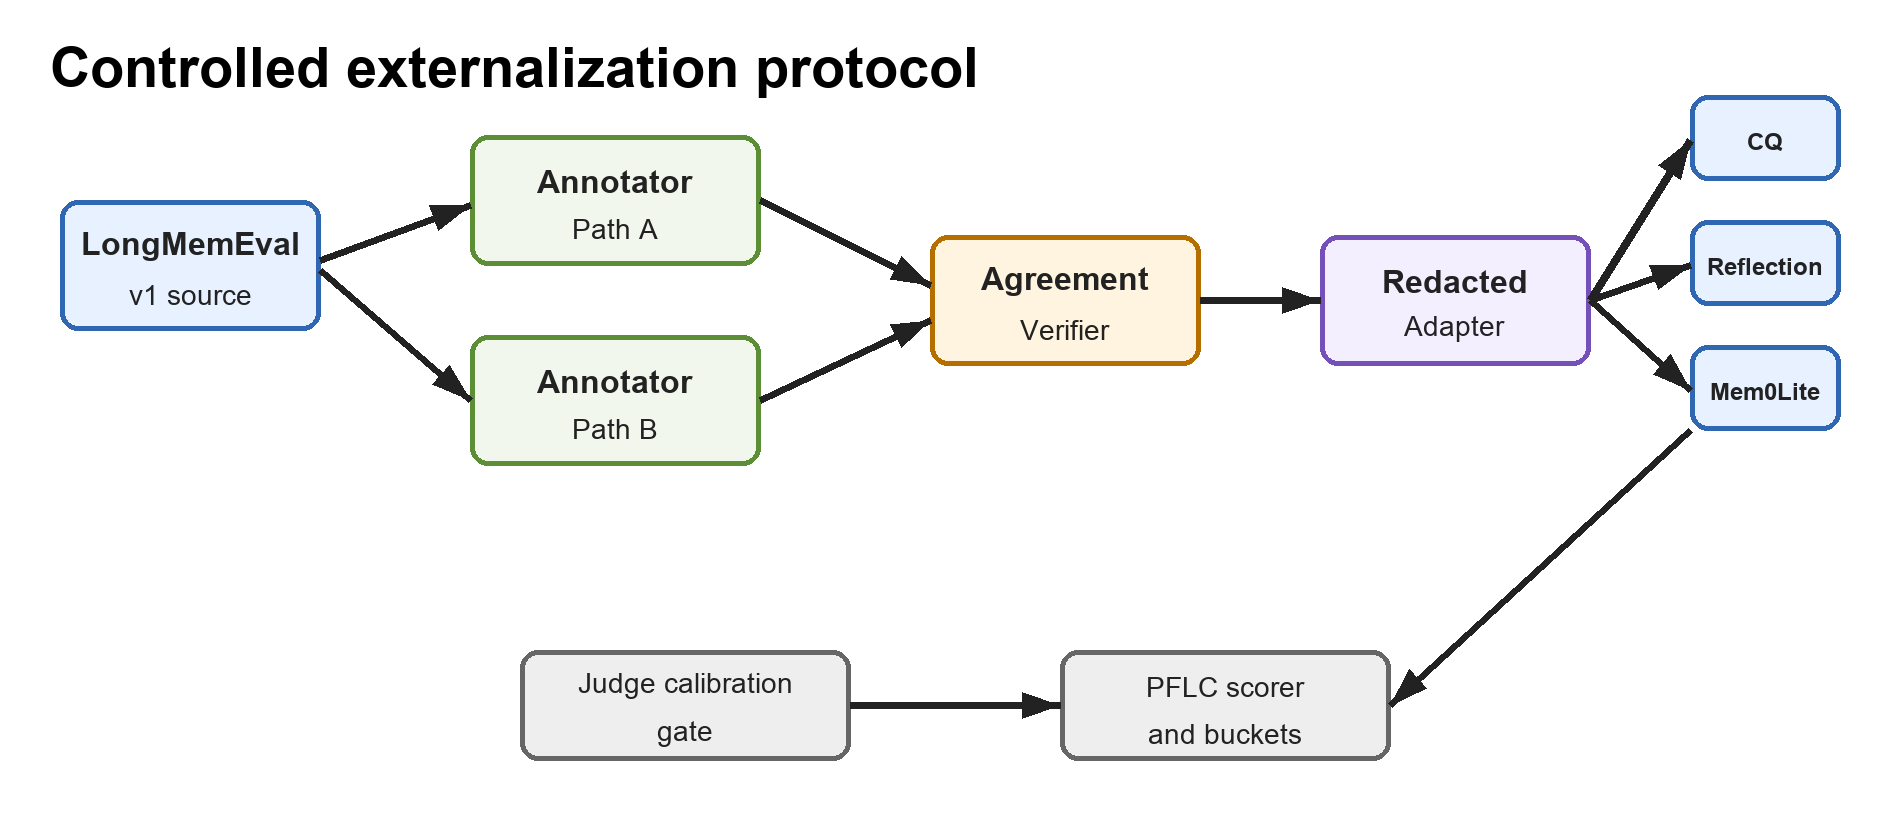
\includegraphics{figures/externalization_protocol.png}
% block in paper/sections/method.tex with
%   % Controlled externalization protocol (replaces externalization_protocol.png).
%
% Usage in main.tex: requires the same preamble additions as
% pflc_formal_gap.tex (tikz + positioning, fit, backgrounds, arrows.meta, calc).
% Replace the existing 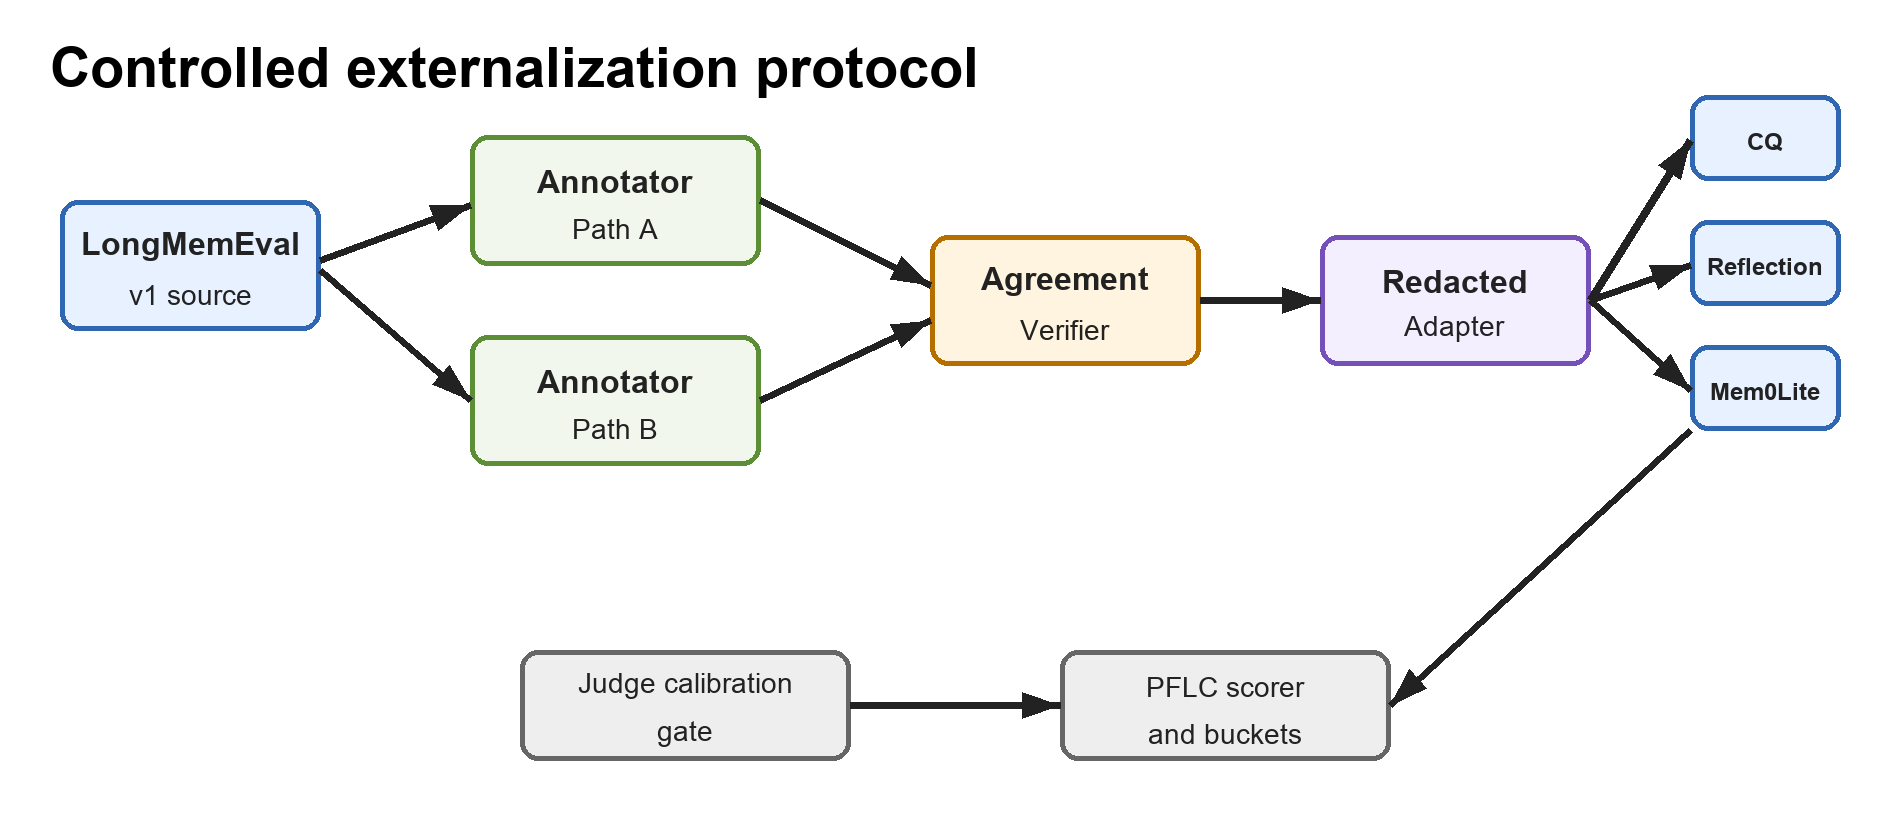
\includegraphics{figures/externalization_protocol.png}
% block in paper/sections/method.tex with
%   % Controlled externalization protocol (replaces externalization_protocol.png).
%
% Usage in main.tex: requires the same preamble additions as
% pflc_formal_gap.tex (tikz + positioning, fit, backgrounds, arrows.meta, calc).
% Replace the existing 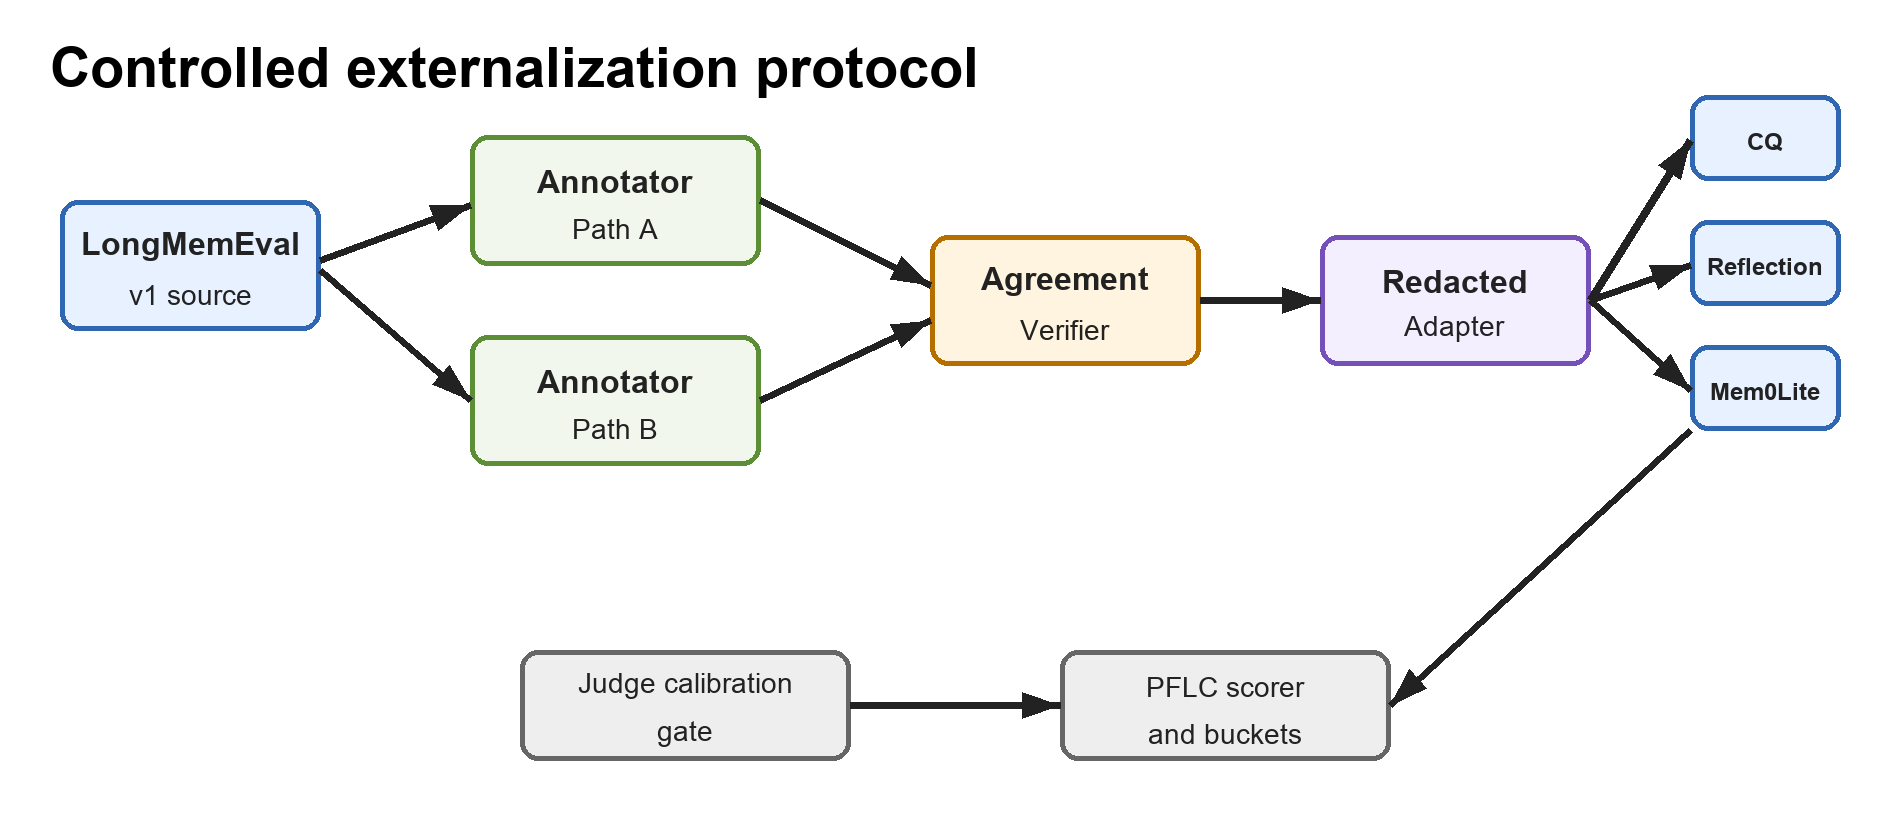
\includegraphics{figures/externalization_protocol.png}
% block in paper/sections/method.tex with
%   \input{figures/externalization_protocol.tex}
%
% Sources for the depicted protocol:
%   docs/fair_stream_externalization_preregistration.md
%   docs/longmemeval_transfer_results.md
%   cq/eval/external/longmemeval/adapter.py
%   cq/eval/external/longmemeval/transfer.py

\begin{figure}[t]
\centering
\resizebox{\linewidth}{!}{%
\begin{tikzpicture}[
  font=\small,
  node distance=6mm,
  stage/.style={
    rounded corners=2pt, draw, line width=0.5pt,
    minimum width=22mm, minimum height=11mm,
    align=center, inner sep=1.5mm,
    font=\small,
  },
  source/.style={stage, draw=blue!60!black, fill=blue!6},
  annot/.style={stage, draw=green!50!black, fill=green!6},
  gate/.style={stage, draw=orange!75!black, fill=orange!7},
  adapt/.style={stage, draw=purple!60!black, fill=purple!6},
  policy/.style={stage, draw=blue!55!black, fill=blue!4, minimum width=18mm, minimum height=8mm},
  judge/.style={stage, draw=gray!70!black, fill=gray!7, font=\footnotesize},
  score/.style={stage, draw=gray!70!black, fill=gray!12, font=\small\bfseries},
  flow/.style={-{Stealth[length=2mm]}, line width=0.6pt},
  side/.style={-{Stealth[length=2mm]}, line width=0.5pt, dashed, gray!70!black},
  label/.style={font=\scriptsize, color=black!65, align=center},
]

% ---- Main pipeline (left to right) ----
\node[source] (src) {LongMemEval\\v1 oracle};

\node[annot, above right=2mm and 9mm of src, anchor=west] (pathA) {Annotator\\Path A};
\node[annot, below right=2mm and 9mm of src, anchor=west] (pathB) {Annotator\\Path B};

\coordinate (verifycenter) at ($(pathA.east)!0.5!(pathB.east)+(15mm,0)$);
\node[gate, anchor=center] (verify) at (verifycenter) {Agreement\\+ verifier};

\node[adapt, right=9mm of verify] (adapter) {Redacted\\adapter (pinned)};

% Three policies stacked
\node[policy, above right=4mm and 10mm of adapter, anchor=west] (cq) {CQ};
\node[policy, right=10mm of adapter] (refl) {Reflection};
\node[policy, below right=4mm and 10mm of adapter, anchor=west] (mem0) {Mem0WritePolicyLite};

\node[score, right=24mm of refl] (scorer) {PFLC scorer\\and bucket};

\node[stage, draw=gray!60!black, fill=gray!4, font=\footnotesize, right=8mm of scorer]
  (cells) {3 sensitivity\\cells};

% ---- Judge calibration gate (precondition above the scorer) ----
\node[judge, above=10mm of scorer] (judge)
  {Judge calibration\\gate (stability pass)};

% ---- Edges ----
\draw[flow] (src.east) to[bend left=18] (pathA.west);
\draw[flow] (src.east) to[bend right=18] (pathB.west);
\draw[flow] (pathA.east) to[bend left=14] (verify.north west);
\draw[flow] (pathB.east) to[bend right=14] (verify.south west);
\draw[flow] (verify.east) -- (adapter.west);
\draw[flow] (adapter.east) to[bend left=10] (cq.west);
\draw[flow] (adapter.east) -- (refl.west);
\draw[flow] (adapter.east) to[bend right=10] (mem0.west);
\draw[flow] (cq.east) to[bend left=8] (scorer.north west);
\draw[flow] (refl.east) -- (scorer.west);
\draw[flow] (mem0.east) to[bend right=8] (scorer.south west);
\draw[flow] (judge.south) -- (scorer.north);
\draw[flow] (scorer.east) -- (cells.west);

% ---- Inline gate annotations (the invariants that fire at each step) ----
\node[label, above=0pt of verify, yshift=8mm] {hidden-answer\\verifier};
\node[label, below=0pt of adapter, yshift=-1mm] {adapter pin SHA};
\node[label, above=2pt of cq] {same candidate stream\\(hash invariant: pass)};

\end{tikzpicture}%
}
\caption{Controlled LongMemEval externalization. The v1 oracle source is
  annotated by two independent paths whose agreement is verified before any
  policy sees data. The redacted adapter strips the gold answer, pins a
  SHA-locked candidate stream, and feeds the same stream to every policy.
  The judge calibration gate must clear stability before scoring runs; the
  PFLC scorer reads policy outputs across three contract-sensitivity cells.}
\label{fig:externalization-protocol}
\end{figure}

%
% Sources for the depicted protocol:
%   docs/fair_stream_externalization_preregistration.md
%   docs/longmemeval_transfer_results.md
%   cq/eval/external/longmemeval/adapter.py
%   cq/eval/external/longmemeval/transfer.py

\begin{figure}[t]
\centering
\resizebox{\linewidth}{!}{%
\begin{tikzpicture}[
  font=\small,
  node distance=6mm,
  stage/.style={
    rounded corners=2pt, draw, line width=0.5pt,
    minimum width=22mm, minimum height=11mm,
    align=center, inner sep=1.5mm,
    font=\small,
  },
  source/.style={stage, draw=blue!60!black, fill=blue!6},
  annot/.style={stage, draw=green!50!black, fill=green!6},
  gate/.style={stage, draw=orange!75!black, fill=orange!7},
  adapt/.style={stage, draw=purple!60!black, fill=purple!6},
  policy/.style={stage, draw=blue!55!black, fill=blue!4, minimum width=18mm, minimum height=8mm},
  judge/.style={stage, draw=gray!70!black, fill=gray!7, font=\footnotesize},
  score/.style={stage, draw=gray!70!black, fill=gray!12, font=\small\bfseries},
  flow/.style={-{Stealth[length=2mm]}, line width=0.6pt},
  side/.style={-{Stealth[length=2mm]}, line width=0.5pt, dashed, gray!70!black},
  label/.style={font=\scriptsize, color=black!65, align=center},
]

% ---- Main pipeline (left to right) ----
\node[source] (src) {LongMemEval\\v1 oracle};

\node[annot, above right=2mm and 9mm of src, anchor=west] (pathA) {Annotator\\Path A};
\node[annot, below right=2mm and 9mm of src, anchor=west] (pathB) {Annotator\\Path B};

\coordinate (verifycenter) at ($(pathA.east)!0.5!(pathB.east)+(15mm,0)$);
\node[gate, anchor=center] (verify) at (verifycenter) {Agreement\\+ verifier};

\node[adapt, right=9mm of verify] (adapter) {Redacted\\adapter (pinned)};

% Three policies stacked
\node[policy, above right=4mm and 10mm of adapter, anchor=west] (cq) {CQ};
\node[policy, right=10mm of adapter] (refl) {Reflection};
\node[policy, below right=4mm and 10mm of adapter, anchor=west] (mem0) {Mem0WritePolicyLite};

\node[score, right=24mm of refl] (scorer) {PFLC scorer\\and bucket};

\node[stage, draw=gray!60!black, fill=gray!4, font=\footnotesize, right=8mm of scorer]
  (cells) {3 sensitivity\\cells};

% ---- Judge calibration gate (precondition above the scorer) ----
\node[judge, above=10mm of scorer] (judge)
  {Judge calibration\\gate (stability pass)};

% ---- Edges ----
\draw[flow] (src.east) to[bend left=18] (pathA.west);
\draw[flow] (src.east) to[bend right=18] (pathB.west);
\draw[flow] (pathA.east) to[bend left=14] (verify.north west);
\draw[flow] (pathB.east) to[bend right=14] (verify.south west);
\draw[flow] (verify.east) -- (adapter.west);
\draw[flow] (adapter.east) to[bend left=10] (cq.west);
\draw[flow] (adapter.east) -- (refl.west);
\draw[flow] (adapter.east) to[bend right=10] (mem0.west);
\draw[flow] (cq.east) to[bend left=8] (scorer.north west);
\draw[flow] (refl.east) -- (scorer.west);
\draw[flow] (mem0.east) to[bend right=8] (scorer.south west);
\draw[flow] (judge.south) -- (scorer.north);
\draw[flow] (scorer.east) -- (cells.west);

% ---- Inline gate annotations (the invariants that fire at each step) ----
\node[label, above=0pt of verify, yshift=8mm] {hidden-answer\\verifier};
\node[label, below=0pt of adapter, yshift=-1mm] {adapter pin SHA};
\node[label, above=2pt of cq] {same candidate stream\\(hash invariant: pass)};

\end{tikzpicture}%
}
\caption{Controlled LongMemEval externalization. The v1 oracle source is
  annotated by two independent paths whose agreement is verified before any
  policy sees data. The redacted adapter strips the gold answer, pins a
  SHA-locked candidate stream, and feeds the same stream to every policy.
  The judge calibration gate must clear stability before scoring runs; the
  PFLC scorer reads policy outputs across three contract-sensitivity cells.}
\label{fig:externalization-protocol}
\end{figure}

%
% Sources for the depicted protocol:
%   docs/fair_stream_externalization_preregistration.md
%   docs/longmemeval_transfer_results.md
%   cq/eval/external/longmemeval/adapter.py
%   cq/eval/external/longmemeval/transfer.py

\begin{figure}[t]
\centering
\resizebox{\linewidth}{!}{%
\begin{tikzpicture}[
  font=\small,
  node distance=6mm,
  stage/.style={
    rounded corners=2pt, draw, line width=0.5pt,
    minimum width=22mm, minimum height=11mm,
    align=center, inner sep=1.5mm,
    font=\small,
  },
  source/.style={stage, draw=blue!60!black, fill=blue!6},
  annot/.style={stage, draw=green!50!black, fill=green!6},
  gate/.style={stage, draw=orange!75!black, fill=orange!7},
  adapt/.style={stage, draw=purple!60!black, fill=purple!6},
  policy/.style={stage, draw=blue!55!black, fill=blue!4, minimum width=18mm, minimum height=8mm},
  judge/.style={stage, draw=gray!70!black, fill=gray!7, font=\footnotesize},
  score/.style={stage, draw=gray!70!black, fill=gray!12, font=\small\bfseries},
  flow/.style={-{Stealth[length=2mm]}, line width=0.6pt},
  side/.style={-{Stealth[length=2mm]}, line width=0.5pt, dashed, gray!70!black},
  label/.style={font=\scriptsize, color=black!65, align=center},
]

% ---- Main pipeline (left to right) ----
\node[source] (src) {LongMemEval\\v1 oracle};

\node[annot, above right=2mm and 9mm of src, anchor=west] (pathA) {Annotator\\Path A};
\node[annot, below right=2mm and 9mm of src, anchor=west] (pathB) {Annotator\\Path B};

\coordinate (verifycenter) at ($(pathA.east)!0.5!(pathB.east)+(15mm,0)$);
\node[gate, anchor=center] (verify) at (verifycenter) {Agreement\\+ verifier};

\node[adapt, right=9mm of verify] (adapter) {Redacted\\adapter (pinned)};

% Three policies stacked
\node[policy, above right=4mm and 10mm of adapter, anchor=west] (cq) {CQ};
\node[policy, right=10mm of adapter] (refl) {Reflection};
\node[policy, below right=4mm and 10mm of adapter, anchor=west] (mem0) {Mem0WritePolicyLite};

\node[score, right=24mm of refl] (scorer) {PFLC scorer\\and bucket};

\node[stage, draw=gray!60!black, fill=gray!4, font=\footnotesize, right=8mm of scorer]
  (cells) {3 sensitivity\\cells};

% ---- Judge calibration gate (precondition above the scorer) ----
\node[judge, above=10mm of scorer] (judge)
  {Judge calibration\\gate (stability pass)};

% ---- Edges ----
\draw[flow] (src.east) to[bend left=18] (pathA.west);
\draw[flow] (src.east) to[bend right=18] (pathB.west);
\draw[flow] (pathA.east) to[bend left=14] (verify.north west);
\draw[flow] (pathB.east) to[bend right=14] (verify.south west);
\draw[flow] (verify.east) -- (adapter.west);
\draw[flow] (adapter.east) to[bend left=10] (cq.west);
\draw[flow] (adapter.east) -- (refl.west);
\draw[flow] (adapter.east) to[bend right=10] (mem0.west);
\draw[flow] (cq.east) to[bend left=8] (scorer.north west);
\draw[flow] (refl.east) -- (scorer.west);
\draw[flow] (mem0.east) to[bend right=8] (scorer.south west);
\draw[flow] (judge.south) -- (scorer.north);
\draw[flow] (scorer.east) -- (cells.west);

% ---- Inline gate annotations (the invariants that fire at each step) ----
\node[label, above=0pt of verify, yshift=8mm] {hidden-answer\\verifier};
\node[label, below=0pt of adapter, yshift=-1mm] {adapter pin SHA};
\node[label, above=2pt of cq] {same candidate stream\\(hash invariant: pass)};

\end{tikzpicture}%
}
\caption{Controlled LongMemEval externalization. The v1 oracle source is
  annotated by two independent paths whose agreement is verified before any
  policy sees data. The redacted adapter strips the gold answer, pins a
  SHA-locked candidate stream, and feeds the same stream to every policy.
  The judge calibration gate must clear stability before scoring runs; the
  PFLC scorer reads policy outputs across three contract-sensitivity cells.}
\label{fig:externalization-protocol}
\end{figure}

%
% Sources for the depicted protocol:
%   docs/fair_stream_externalization_preregistration.md
%   docs/longmemeval_transfer_results.md
%   cq/eval/external/longmemeval/adapter.py
%   cq/eval/external/longmemeval/transfer.py

\begin{figure}[t]
\centering
\resizebox{\linewidth}{!}{%
\begin{tikzpicture}[
  font=\small,
  node distance=6mm,
  stage/.style={
    rounded corners=2pt, draw, line width=0.5pt,
    minimum width=22mm, minimum height=11mm,
    align=center, inner sep=1.5mm,
    font=\small,
  },
  source/.style={stage, draw=blue!60!black, fill=blue!6},
  annot/.style={stage, draw=green!50!black, fill=green!6},
  gate/.style={stage, draw=orange!75!black, fill=orange!7},
  adapt/.style={stage, draw=purple!60!black, fill=purple!6},
  policy/.style={stage, draw=blue!55!black, fill=blue!4, minimum width=18mm, minimum height=8mm},
  judge/.style={stage, draw=gray!70!black, fill=gray!7, font=\footnotesize},
  score/.style={stage, draw=gray!70!black, fill=gray!12, font=\small\bfseries},
  flow/.style={-{Stealth[length=2mm]}, line width=0.6pt},
  side/.style={-{Stealth[length=2mm]}, line width=0.5pt, dashed, gray!70!black},
  label/.style={font=\scriptsize, color=black!65, align=center},
]

% ---- Main pipeline (left to right) ----
\node[source] (src) {LongMemEval\\v1 oracle};

\node[annot, above right=2mm and 9mm of src, anchor=west] (pathA) {Annotator\\Path A};
\node[annot, below right=2mm and 9mm of src, anchor=west] (pathB) {Annotator\\Path B};

\coordinate (verifycenter) at ($(pathA.east)!0.5!(pathB.east)+(15mm,0)$);
\node[gate, anchor=center] (verify) at (verifycenter) {Agreement\\+ verifier};

\node[adapt, right=9mm of verify] (adapter) {Redacted\\adapter (pinned)};

% Three policies stacked
\node[policy, above right=4mm and 10mm of adapter, anchor=west] (cq) {CQ};
\node[policy, right=10mm of adapter] (refl) {Reflection};
\node[policy, below right=4mm and 10mm of adapter, anchor=west] (mem0) {Mem0WritePolicyLite};

\node[score, right=24mm of refl] (scorer) {PFLC scorer\\and bucket};

\node[stage, draw=gray!60!black, fill=gray!4, font=\footnotesize, right=8mm of scorer]
  (cells) {3 sensitivity\\cells};

% ---- Judge calibration gate (precondition above the scorer) ----
\node[judge, above=10mm of scorer] (judge)
  {Judge calibration\\gate (stability pass)};

% ---- Edges ----
\draw[flow] (src.east) to[bend left=18] (pathA.west);
\draw[flow] (src.east) to[bend right=18] (pathB.west);
\draw[flow] (pathA.east) to[bend left=14] (verify.north west);
\draw[flow] (pathB.east) to[bend right=14] (verify.south west);
\draw[flow] (verify.east) -- (adapter.west);
\draw[flow] (adapter.east) to[bend left=10] (cq.west);
\draw[flow] (adapter.east) -- (refl.west);
\draw[flow] (adapter.east) to[bend right=10] (mem0.west);
\draw[flow] (cq.east) to[bend left=8] (scorer.north west);
\draw[flow] (refl.east) -- (scorer.west);
\draw[flow] (mem0.east) to[bend right=8] (scorer.south west);
\draw[flow] (judge.south) -- (scorer.north);
\draw[flow] (scorer.east) -- (cells.west);

% ---- Inline gate annotations (the invariants that fire at each step) ----
\node[label, above=0pt of verify, yshift=8mm] {hidden-answer\\verifier};
\node[label, below=0pt of adapter, yshift=-1mm] {adapter pin SHA};
\node[label, above=2pt of cq] {same candidate stream\\(hash invariant: pass)};

\end{tikzpicture}%
}
\caption{Controlled LongMemEval externalization. The v1 oracle source is
  annotated by two independent paths whose agreement is verified before any
  policy sees data. The redacted adapter strips the gold answer, pins a
  SHA-locked candidate stream, and feeds the same stream to every policy.
  The judge calibration gate must clear stability before scoring runs; the
  PFLC scorer reads policy outputs across three contract-sensitivity cells.}
\label{fig:externalization-protocol}
\end{figure}
